\usetikzlibrary{mindmap,trees}
\titleSlide
\inuitsSlide

\frame{%
    \frametitle{whoami}
    \framesubtitle{Julien Pivotto}
    \begin{itemize}
        \item{System administrator at {\inuits{}inuits\small.eu}}
        \item{Git user for 5+ years}
        \item{DevOps believer}
        \item{Open-source defender since 2004}
        \olditem{\textit{\ctr{@roidelapluie}} \ctr{on irc/twitter/github}}
    \end{itemize}
}

\frame{%

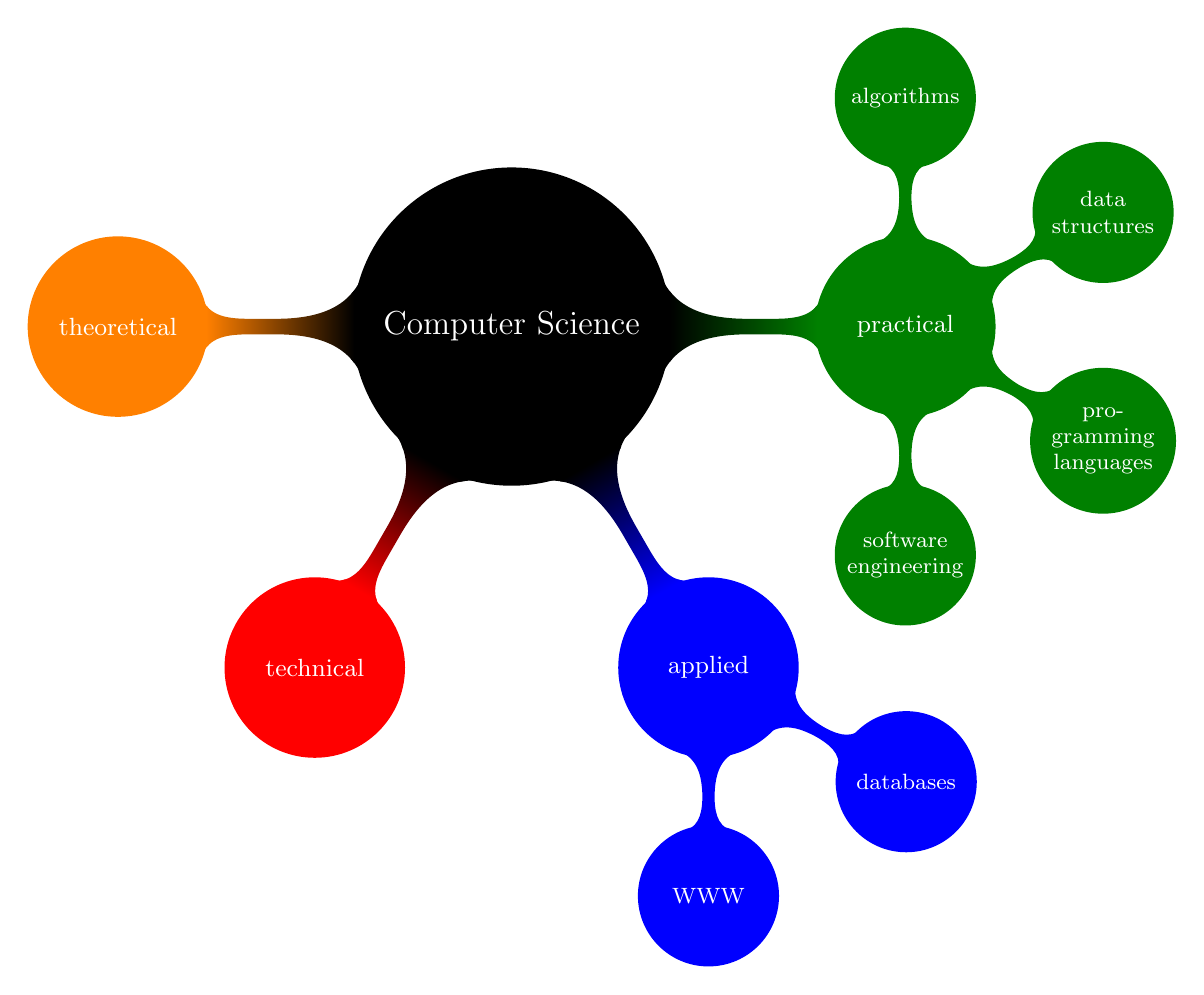
\begin{tikzpicture}
    \path[mindmap,concept color=black,text=white]
    node[concept] {Computer Science}
    [clockwise from=0]
    child[concept color=green!50!black] {
        node[concept] {practical}
        [clockwise from=90]
        child { node[concept] {algorithms} }
        child { node[concept] {data structures} }
        child { node[concept] {pro\-gramming languages} }
        child { node[concept] {software engineer\-ing} }
    }  
    child[concept color=blue] {
        node[concept] {applied}
        [clockwise from=-30]
        child { node[concept] {databases} }
        child { node[concept] {WWW} }
    }
    child[concept color=red] { node[concept] {technical} }
    child[concept color=orange] { node[concept] {theoretical} };
    \end{tikzpicture}
}


% quickintro
% basics
% commit message vs project management
% git blame
% git stash
% workflows
% git squash
% git merge

\thankyouSlide
\renewcommand{\insertLogo}{}
\contactSlide

